\documentclass[12pt, a4paper]{report}

%%%%%%%%%%%%%%%%%%%%%%%%%%%%%%%%%
% PACKAGE IMPORTS
%%%%%%%%%%%%%%%%%%%%%%%%%%%%%%%%%

% \usepackage[T1]{fontenc}
% \usepackage[utf8]{inputenc}

\usepackage[style=science]{biblatex}
\addbibresource{aohashes.bib}

\usepackage[tmargin=3cm,rmargin=1in,lmargin=1in,margin=0.85in,bmargin=3cm]{geometry}
\usepackage{amsmath,amsfonts,amsthm,amssymb,mathtools}
\usepackage{bookmark}
\usepackage{hyperref}
\hypersetup{
	colorlinks=true,
  % allcolors=fg,
  linkcolor=fg,
  citecolor=cyan,
	bookmarksnumbered=true,
	bookmarksopen=true
}
\usepackage[most,many,breakable]{tcolorbox}
\usepackage{colortbl}
\usepackage{tikz}
\usetikzlibrary{arrows,calc,shadows.blur}
\usepackage{pgfplots}
\pgfplotsset{compat=1.5}
\usepackage{float}
\usepackage{graphicx}
\graphicspath{ {figures/} }
\usepackage{caption}
\usepackage{subcaption}

\usepackage{listings}
\lstdefinestyle{scripts}{
    backgroundcolor=\color{bg},   
    commentstyle=\color{gray},
    basicstyle=\ttfamily\footnotesize,
    breakatwhitespace=false,         
    breaklines=true,                 
    captionpos=b,                    
    keepspaces=true,                 
    showspaces=false,                
    showstringspaces=false,
    showtabs=false,                  
    tabsize=2
}

\lstset{style=scripts}

%%%%%%%%%%%%%%%%%%%%%%%%%%%%%%
% COLORS
%%%%%%%%%%%%%%%%%%%%%%%%%%%%%%

\definecolor{bg}{HTML}{F2F2F2}
\definecolor{fg}{HTML}{282828}

%%%%%%%%%%%%%%%%%%%%%%%%%%%%
% MARGINS
%%%%%%%%%%%%%%%%%%%%%%%%%%%%

\setlength{\parindent}{0pt}

% change default chapter distance
\makeatletter
% --- Patch \chapter
\patchcmd{\@makechapterhead}{50\p@}{\chapheadtopskip}{}{}
\patchcmd{\@makechapterhead}{20\p@}{\chapheadsep}{}{}
\patchcmd{\@makechapterhead}{40\p@}{\chapheadbelowskip}{}{}
% --- Patch \chapter*
\patchcmd{\@makeschapterhead}{50\p@}{\chapheadtopskip}{}{}
\patchcmd{\@makeschapterhead}{40\p@}{\chapheadbelowskip}{}{}
\makeatother
% Set new lengths
\newlength{\chapheadtopskip}\setlength{\chapheadtopskip}{0pt}
\newlength{\chapheadsep}\setlength{\chapheadsep}{15pt}
\newlength{\chapheadbelowskip}\setlength{\chapheadbelowskip}{25pt}

%================================
% NOTE BOX
%================================

\tcbuselibrary{skins}
\newtcolorbox{note}[1][]{%
	enhanced jigsaw,
	colback=bg,
	colframe=fg,
	size=small,
	boxrule=1pt,
  title=\textbf{\textbf{NOTE:}},
	before upper = \tcbtitle\par,
	detach title,
	coltitle=fg,
	breakable,
	drop shadow=fg!50!bg,
	#1,
}

%%%%%%%%%%%%%%%%%%%%%%%%%%%%%%
% COMMANDS
%%%%%%%%%%%%%%%%%%%%%%%%%%%%%%

\renewcommand{\leq}{\leqslant}
\renewcommand{\geq}{\geqslant}

%%%%%%%%%%%%%%%%%%%%%%%%%%%%%%%%%%%%%%%%%%%
% TABLE OF CONTENTS
%%%%%%%%%%%%%%%%%%%%%%%%%%%%%%%%%%%%%%%%%%%

\usepackage{titletoc}
\contentsmargin{0cm}
\titlecontents{part}[-1pc]
{\addvspace{50pt}%
	
\begin{tikzpicture}[remember picture, overlay]%
		\draw[fill=fg!85,draw=fg!85] (-4.5,-0.2) rectangle (-0.15,0.55);%
		\pgftext[left,x=-1.6cm,y=0.15cm]{\color{bg}\Large\sc\bfseries Part};%
	\end{tikzpicture}\color{fg}\large\sc\bfseries}
{}
{}
{}
\titlecontents{chapter}[5pc]
{\addvspace{30pt}%
	
\begin{tikzpicture}[remember picture, overlay]%
		\draw[fill=fg!85,draw=fg!85] (-3.6,-0.2) rectangle (-0.12,0.55);%
		\pgftext[left,x=-3.5cm,y=0.15cm]{\color{bg}\Large\sc\bfseries Chapter\ \thecontentslabel};%
	\end{tikzpicture}\color{fg}\large\sc\bfseries}%
{}
{}
{\;\titlerule\;\large\sc\bfseries Page \thecontentspage
	\begin{tikzpicture}[remember picture, overlay]
		\draw[fill=fg,draw=fg] (4pt,0.2pt) rectangle (4,0.2pt);
	\end{tikzpicture}}%
\titlecontents{section}[5pc]
{\addvspace{2pt}}
{\contentslabel[\thecontentslabel]{2pc}}
{}
{\hfill\small \thecontentspage}
[]
\titlecontents{subsection}[5pc]
{\addvspace{2pt}}
{\scriptsize$\bullet$\quad\small}
{}
{\hfill\small}
% {\hfill\small \thecontentspage}
[]

\makeatletter
\renewcommand{\tableofcontents}{%
	\chapter*{%
	  \vspace*{-20\p@}%
	  \begin{tikzpicture}[remember picture, overlay]%
		  \pgftext[right,x=16.7cm,y=0.2cm]{\color{fg!85}\Huge\sc\bfseries \contentsname};%
		  \draw[fill=fg!85,draw=fg!85] (14.6,-0.65) rectangle (20,1);%
		  \clip (14.6,-0.65) rectangle (20,1);
		  \pgftext[right,x=16.7cm,y=0.2cm]{\color{bg}\Huge\sc\bfseries \contentsname};%
	  \end{tikzpicture}}%
	\@starttoc{toc}}
\makeatother


\title{{\textbf{AOHashes}}\\[20pt]\textsl{AO privacy-friendly primitives testing\\over Dusk-\textsf{Plonk} ZK library}}
\author{\Large{Filippo Merlo}}
\date{\textit{March 2025}}
\begin{document}

\maketitle
\newpage
\pdfbookmark[section]{\contentsname}{toc}
\tableofcontents
\pagebreak

\begin{abstract}
This paper presents a comparative analysis of several Arithmetization-Oriented (AO) cryptographic primitives, designed to enhance the efficiency of Zero-Knowledge (ZK) proofs.
AO primitives are optimized to work with constraint-based ZK proof systems like \textsf{Plonk}, which are widely used for privacy-focused applications such as blockchain and secure authentication.

By implementing these primitives in the Rust programming language and testing them with the Dusk Network’s \textsf{Plonk} library, we aim to assess their performance in terms of computational speed, constraint complexity and proof generation efficiency.
The primitives evaluated include \texttt{GMiMC}, \textsc{Poseidon}, \texttt{Rescue}, \texttt{Rescue-Prime}, \textsc{Griffin}, \texttt{Anemoi} and \texttt{Arion}, each with unique design strategies that balance the trade-offs between security, efficiency and polynomial degree.

Our analysis provides a clear comparison of how these primitives perform under various conditions, highlighting their strengths and limitations.
We also discuss which primitives may be best suited for specific applications based on their stability, computational overhead or adaptability to different field sizes and security levels.
By shedding light on these performance characteristics, we hope to guide future optimizations and inspire new cryptographic designs that can further enhance the efficiency ZK proof systems.
\end{abstract}

\chapter{Introduction}\label{chap:intro}

In recent years, the field of cryptography has seen a surge of interest in Zero-Knowledge (ZK) proofs, which allows one party (the prover) to prove the validity of a computation to another party (the verifier) without revealing any underlying data.
This unique property makes ZK proofs particularly valuable in applications where privacy and data security are crucial, such as blockchain technology, authentication systems and secure financial transactions.

Among the various types of ZK proofs, a special category known as non-interactive proofs has gained popularity.
Unlike interactive ZK proofs, non-interactive proofs do not require communication between the prover and the verifier, making them ideal for decentralized environments like blockchains.

This paper focuses on a specific type of non-interactive ZK proof system called \textsf{Plonk}~\cite{plonk}, which belongs to the SNARK\footnote{Succinct Non-interactive ARguments of Knowledge} family.
\textsf{Plonk} proofs are based on arithmetic circuits, which are translated into constraints and finally represented as polynomials that will be evaluated by the verifier.
This structure, even if it at first glance seems complex and computationally heavy, in reality is very efficient and powerful for solving ZK proof problems.

However, one challenge with ZK proof systems including \textsf{Plonk} is that traditional cryptographic primitives are not well-suited to work within these terms and structures, losing all their efficiency from a performance point of view.
To address this, researchers have developed a new class of cryptographic primitives designed specifically for this purpose, known as Arithmetization-Oriented (AO) primitives.
These AO primitives aim to maximize the performance of ZK proofs by minimizing the computational overhead associated with constraints, particularly when performing basic operations like addition and multiplication.

In this paper, we explore and evaluate several of the latest AO primitives that have been proposed and published in these last years through a Rust programming language implementation and the testing with the Dusk Network's \textsf{Plonk} ZK library~\cite{dusk-plonk}.
Our goal is to compare these primitives based on their performance, efficiency and suitability for different use cases.
By highlighting their strengths and weaknesses, we aim to provide valuable insights for developers and researchers interested in optimizing ZK proof systems and designing new cryptographic solutions.

\chapter{Overview}\label{chap:overview}

As mentioned in the introductory \autoref{chap:intro}, the primitives that have been tested in this project are Arithmetization-Oriented and this is because for Zero-Knowledge proofs plain evaluation is important, but proofs generation and verification is even more critical, and this design provides an efficient solution for performing both operations.
Another important aspect of AO primitives is that they are suitable for a vast number of field sizes and security levels, making them very elastic and adaptable to different scenarios and applications.
However, as we will evidence from this paper's results, the design of these primitives can severely affect the computational time of generating and verifying proofs even though the same environment is provided and the same instances are used.

Because the Dusk Network team provides a library that implements the \textsf{Plonk} system~\cite{dusk-plonk}, plus they also implement the primitive \textsc{Poseidon}~\cite{dusk-poseidon}, we have decided to implement all the remaining primitives using the same programming language used for these two implementations (\textsl{i.e.} Rust) in a single project, in order to have the same baseline for all the primitives and being able to conduct a fair comparison between them, minimizing potential sources of errors in our final results.

For this reason we have chosen to work on only one the BLS12-381 elliptic curve, with\\ $p = 52435875175126190479447740508185965837690552500527637822603658699938581184513$.

\section{Primitives}\label{sec:primitives}

The primitives that have been implemented and tested in this project are:
\begin{itemize}
  \item \texttt{GMiMC}~\cite{gmimc}
  \item \textsc{Poseidon}~\cite{poseidon}
  \item \texttt{Rescue}~\cite{rescue}
  \item \texttt{Rescue-Prime}~\cite{rescue-prime}
  \item \textsc{Griffin}~\cite{griffin}
  \item \texttt{Anemoi}~\cite{anemoi}
  \item \texttt{Arion}~\cite{arion}
\end{itemize}

We can split them into two categories: in the \textit{first category} we found those that have been designed for maintaining the \textbf{degree of polynomials} as \textbf{low} as possible, while having a high number of rounds to achieve a minimum level of bits security, which are \texttt{GMiMC}, \textsc{Poseidon}, \texttt{Rescue} and \texttt{Rescue-Prime}, while in the \textit{second} one has been used the opposite strategy, \textsl{i.e.} achieving efficiency maintaining a \textbf{low number of rounds}, but increasing exponentially the polynomial degree with the introduction of inverse power permutations, and these primitives are \textsc{Griffin}, \texttt{Anemoi} and \texttt{Arion}.

\subsection{\texttt{GMiMC}}\label{subsec:gmimc}

The first function implemented in this project it has been \texttt{GMiMC}\footnote{Generalized MiMC}: a hash function based on unbalanced Feistel networks with a low multiplicative complexity that suits well ZK-SNARK applications.
The mapping used in the Feistel networks is $x \rightarrow x^d$, which is a design idea by Nyberg and Knudsen, that has been shown it leads to efficient instatiations for SNARKs~\cite{mimc}. Among the available Feistel network modes, for this project we implemented the ERF\footnote{Expanding Round Function} variant, which schema is depicted in \autoref{fig:gmimc}.

\begin{figure}[H]
  \begin{center}
    \includegraphics[width=0.35\textwidth]{gmimc/round.png}
  \end{center}
  \caption{Single round of $\texttt{GMiMC}_\texttt{ERF}$~\cite[Fig.~2]{gmimc}.}\label{fig:gmimc}
\end{figure}

As it is possible to deduct from the above schema, a single $\texttt{GMiMC}_\texttt{ERF}$ round is composed of the following operations:
\begin{itemize}
  \item Computation of $y = F(x_0): x_0 \rightarrow x_0^d$, where $x_0$ is the first element of the state;
  \item XOR addition between each element of the state except the first one, and the output $y$ of $F$;
  \item Left-rotation of the state by one position.
\end{itemize}

Some common instatiations of \texttt{GMiMC} to achieve the minimum security of 128 bits over the curve BLS12-381 are shown in \autoref{tab:gmimcinstances}, while the formula used to compute the minimum number of rounds $n$~\cite[Tab.~2,Tab.~3]{gmimc} against some common cryptographic attacks is:
\begin{equation}
  n = \max \left\{ n_{\text{Int}}, n_{\text{HighOrd}}, n_{\text{RTDif}} \right\},
  \label{eq:gmimcrounds}
\end{equation}
where
\begin{align}
  n_{\text{Int}} & = \left \lceil 2 \cdot \log_d(2) \cdot \log_2(p) \right\rceil + 2t ,\\[10pt]
  n_{\text{HighOrd}} & = 2 + 2t + \left \lceil 2 \cdot \log_d(t) \right\rceil ,\\[6pt]
  n_{\text{RTDif}} & = 2 + \left \lceil (t^2 + t) \cdot \frac{\log_2(p)}{2 \cdot (\log_2(p) - 1)} \right\rceil ,
\end{align}
where $t$ is the state width, $d$ is the exponent of the mapping function $F$ (in our chase 5) and $p$ is the prime used for our curve.

\begin{table}[H]
  \caption{$\texttt{GMiMC}_\texttt{ERF}$ instances for $d = 5$.}\label{tab:gmimcinstances}
  \begin{center}
    \begin{tabular}{|l|c|c|c|c|c|}
      \hline
      $t$ state width & 3 & 4 & 5 & 6 & 8 \\
      \hline
      $n$ rounds & 328 & 330 & 332 & 334 & 338 \\
      \hline
    \end{tabular}
  \end{center}
\end{table}
\subsection{\textsc{Poseidon}}\label{subsec:poseidon}

\textsc{Poseidon} is a \textbf{sponge function}~\cite{sponge} whose inner permutation function named $\textsc{Poseidon}^\pi$ is an unkeyed version of the \textsc{Hades} strategy~\cite{hades}.
The $\textsc{Poseidon}^\pi$ permutation exploits two round functions, respectively denoted as \textit{full} and \textit{partial}, and their difference resides in how the S-Box\footnote{Substitution Box} is applied.
Precisely, in the full round version the S-Box is applied to each element of the state, while in the partial one only to the last element of the state. 
The decision to opt for this design strategy in the permutation function is attributable to the goal of improving \textsc{Poseidon}'s performance even with a high number of rounds, by lightening the final computational cost with the removal of some S-Boxes.
\begin{note}
It is important to notice that $\textsc{Poseidon}^\pi$ can be adjusted to use only full rounds and achieving in this way a greater level of security.
However, the opposite, \textsl{i.e.} using only partial rounds, is strongly discouraged because to achieve a minimum level of security a minimal amount of full rounds are still required, where the exact value depends on the size $t$ of the state.
\end{note}

A single round is composed of the following concatenation of functions:
\begin{itemize}
  \item \textit{AddRoundConstant} (ARC): a constant $c_r$, where $r$ is the value of the round, is added to each value of state;
  \item \textit{S-Box} (S): the input is exponentiated to an exponent $d$ where $d \ge 3$ and also $d$ is co-prime with $p-1$. This function is applied singularly to each/last element of the state, depending on the type of round;
  \item \textit{MixLayer} (M): matrix-vector multiplication between a fixed matrix and the state, where the matrix is a square MDS\footnote{Maximum Distance Separable} matrix chosen such that no subspace trail with inactive/active S-Boxes can be set up for more than $t-1$ rounds, with $t$ the size of the state.
\end{itemize}

In \autoref{fig:poseidon} is shown the complete structure of the $\textsc{Poseidon}^\pi$ function, while in \autoref{tab:poseidoninstances} are collected the most commonly used instantiations for \textsc{Poseidon}~\cite[Tab.2]{poseidon}.

\begin{figure}[H]
  \begin{center}
      \includegraphics[width=0.55\textwidth]{poseidon/permutation.png}
  \end{center}
  \caption{$\textsc{Poseidon}^\pi$ permutation function~\cite[Fig.~2]{poseidon}.}\label{fig:poseidon}
\end{figure}

\begin{table}[H]
  \caption{\textsc{Poseidon} instances for $d=5$~\cite[Tab.~2]{poseidon}.}\label{tab:poseidoninstances}
  \begin{center}
    \begin{tabular}{|l|c|c|}
      \hline
      $t$ state width & 2/3 & 4/5/6/8 \\
      \hline
      $n_f$ full rounds & 8 & 8 \\
      \hline
      $n_p$ partial rounds & 57 & 60 \\
      \hline
    \end{tabular}
  \end{center}
\end{table}

\subsection{\texttt{Rescue}}\label{subsec:rescue}

The \texttt{Rescue} primitive is a sponge function based on the \texttt{Marvellous} design strategy and the focus of the authors of this primitive was realizing a secure and robust function, rather than an efficient one, while keeping a simple structure.
For this purpose, they proposed the \texttt{Marvellous} strategy which is a SPN\footnote{Substitution-Permutation Network} round function, where each round is split into two phases and each phase is the composition of different operations.

A single round is organized as follows:
\begin{itemize}
  \item \textbf{First phase}
  \begin{itemize}
    \item \textit{Inverse S-Box} ($\text{S}^{-1}$): application of the inverse power map $x_i \rightarrow x_i^{\frac{1}{d}}$ to each element of the state;
    \item \textit{MixLayer} (M): matrix-vector multiplication between an MDS matrix and the state;
    \item \textit{AddRoundConstant} (ARC): addition of a constant $c^r_i$ to each element of the state $x_i$ where $0 \le i < t$ is the index of the elements of the states and $r$ is the round value and $t$ the state width;
  \end{itemize}
  \newpage
  \item \textbf{Second phase}
  \begin{itemize}
    \item \textit{S-Box} (S): application of the power map $x_i \rightarrow x_i^d$ to each element of the state;
    \item \textit{MixLayer} (M): matrix-vector multiplication with the same MDS matrix of the first phase;
    \item \textit{AddRoundConstant} (ARC): addition of another set of constants $c^r_{t+i}$ to each element of the state (it has been used the same notation of the first phase).
  \end{itemize}
\end{itemize}

The round function of \texttt{Rescue} is summarized in \autoref{fig:rescue}:
\begin{figure}[H]
  \begin{center}
    \hspace{30pt}
    \includegraphics[width=0.43\textwidth]{rescue/round.png}
  \end{center}
  \caption{$r$-th round of \texttt{Marvellous} permutation.}\label{fig:rescue}
\end{figure}

The minimum number of rounds $n$ needed to achieve 128 bits of security is computed with the following formula~\cite[Tab.~1]{rescue}:
\begin{equation}
  n = 2 \cdot \max \left\{l_0, l_1, 5 \right\},
  \label{eq:rescuerounds}
\end{equation}
where
\begin{align}
  l_0 & = \max \left\{ n_{\text{Dif}}, n_{\text{HighOrd}}, n_{\text{Int}} \right\} , \\
  l_1 & = \min_N \text{ subject to } \left( \begin{array}{c} [(16N - 1) \cdot t + 1]/4 \\ 2t \cdot N \end{array}\right)^2 ,
\end{align}
which respectively are 
\begin{itemize}
  \item $l_0$ the maximum number of rounds that can be generically attacked via Differential or Linear Cryptanalysis, High Order Differentials or Interpolation;
  \item $l_1$ the minimum number of rounds to be secure against a Gr\"obner basis cryptanalysis attack.
\end{itemize}

Therefore, the most common instantiations of \texttt{Rescue} computed using the just explained formula are shown here in \autoref{tab:rescueinstances}:
\begin{table}[H]
  \caption{\texttt{Rescue} instances for $d = 5$.}\label{tab:rescueinstances}
  \begin{center}
    \begin{tabular}{|l|c|c|c|c|}
      \hline
      $t$ state width & 3 & 4 & 5 & 6/8 \\
      \hline
      $n$ rounds & 14 & 11 & 9 & 8 \\
      \hline
    \end{tabular}
  \end{center}
\end{table}

\subsection{\texttt{Rescue-Prime}}\label{subsec:rescueprime}

The hash function \texttt{Rescue-Prime} has the same general underlying structure of \texttt{Rescue}~(\autoref{subsec:rescue}), but with minor adjustments to simplify the implementation, which are:
\begin{itemize}
  \item Simplification of the round constants' derivation function;
  \item Reduction of the security margin to its half (\textsl{i.e.} from $100\%$ to $50\%$);
  \item Flipping the order of the S-Boxes.
\end{itemize}

The authors decided to not override the previous \texttt{Rescue} hash function, but to deploy these changes in a new version and to do so they decided to give it a new name to maintain a clear distinction between the two versions.
In fact, even the inner permutation function changed name to \texttt{Rescue-XLIX}\footnote{Rescue Forty-nine}.

The round function described for \texttt{Rescue} is still valid for \texttt{Rescue-Prime}, but with the changes mentioned above, \textsl{i.e.} swap of the S-Boxes order.

Because the general structure is the same, also the number of rounds and state width are the same shown in \autoref{tab:rescueinstances}.

\subsection{\textsc{Griffin}}\label{subsec:griffin}

This primitive, born from the results collected by the designs of \texttt{GMiMC} and \texttt{Rescue}, is the union of both SPN and Feistel networks schemes.
The structure on which \textsc{Griffin} has been built upon is called \textit{Horst} and is a revised version of Feistel networks, that grants a more robust defense against algebraic attacks \textsl{e.g.} Gr\"obner basis attacks.

The internal permutation function implemented for \textsc{Griffin} is called \textsc{Griffin-$\pi$} and has been designed to lower the minimum number of rounds while maintain a certain security level; this is achieved by the introduction of an exponentiation of very high degree on only one element of the state. This choice allows reducing the number of rounds without increasing too much the computational complexity and the number of constraints in the ZK proof.

\newpage
A single round of the permutation function \textsc{Griffin-$\pi$} is organized as follows:
\begin{itemize}
  \item \textit{S-Box} (S): depending on the element's position, the transformation of the \textit{S-Box} is different and its formula~\cite[Eq.~6]{griffin} is
  \begin{equation}
    y_i = \left\{
      \begin{array}{ll}
        x_0^{1/d} & \text{if } i = 0; \\
        x_1^{d} & \text{if } i = 1; \\
        x_i \cdot ((L_i^2 + \alpha_i \cdot L_i + \beta_i) & \text{otherwise}.
      \end{array}
    \right.,
    \label{eq:griffinsbox}
  \end{equation}
  where
  \begin{equation}
    L_i = \left\{
      \begin{array}{ll}
        (i-1) \cdot y_0 + y_1 & \text{if } i = 2; \\
        (i-1) \cdot y_0 + y_1 + x_{i-1} & \text{otherwise}.
      \end{array}
    \right.,
    \label{eq:griffinli}
  \end{equation}
  and $\alpha_i$,$\beta_i$ are constants generated \textsl{s.t.} $\alpha_i^2 - 4 \cdot \beta_i$ is a quadratic non-residue modulo $p$;
  \item \textit{MixLayer} (M): matrix-vector multiplication between an MDS matrix and the state;
  \item \textit{AddRoundConstant} (ARC): addition of the round constant $c^r$, where $r$ is the round value, to each element of the state. In the last round (\textsl{i.e.} $n-1$), the round constant is equal to 0, thus this operation can be omitted in the implementation.
\end{itemize}

Before computing the \textsc{Griffin-$\pi$} permutation function on the needed rounds, the state needs to be initialized with the application of the \textit{MixLayer} matrix-vector multiplication for an increased diffusion and better security.
Furthermore, the permutation \textsc{Griffin-$\pi$} can be used with \textsc{Griffin} in sponge as well as in a compression mode, interchangeably. 

The complete \textsc{Griffin-$\pi$} function has been schematized in the following \autoref{fig:griffin}:
\begin{figure}[H]
  \begin{center}
    \includegraphics[width=0.93\textwidth]{griffin/permutation.png}
  \end{center}
  \caption{\textsc{Griffin-$\pi$} permutation function~\cite[Fig.~2]{griffin}.}\label{fig:griffin}
\end{figure}

In the \autoref{tab:griffininstances} are provided the most common instantiations of \textsc{Griffin}, where the minimum number of rounds $n$ is computed with the following formula:
\begin{equation}
  n \ge \left\lceil 1.2 \cdot \max \left\{6, \left\lceil \frac{2.5 \cdot \kappa}{\log_2(p) - \log_2(d-1)} \right\rceil, 1 + n_{GB} \right\} \right\rceil ,
  \label{eq:griffinrounds}
\end{equation}
where $\kappa$ is the bits' security level (in our case 128), $p$ is the prime used for the curve, $d$ is the exponent of the S-Box and $n_{GB}$ is the number of rounds needed to defend against Gr\"obner basis attacks.

\begin{table}[H]
  \caption{\textsc{Griffin} instances for $d = 5$~\cite[Tab.~2]{griffin}.}\label{tab:griffininstances}
  \begin{center}
    \begin{tabular}{|l|c|c|c|}
      \hline
      $t$ state width & 3 & 4 & 8 \\
      \hline
      $n$ rounds & 14 & 11 & 9 \\
      \hline
    \end{tabular}
  \end{center}
\end{table}

\subsection{\texttt{Anemoi}}\label{subsec:anemoi}

To improve the efficiency in terms of \textbf{evaluation} and \textbf{verification} of zero-knowledge proof circuits, the primitive \texttt{Anemoi} has been designed exploiting the strength of \textbf{CCZ-equivalence}.
\texttt{Anemoi} is a sponge function whose inner permutation doesn't implement the usual S-Box structure, but instead a new design called \texttt{Flystel}.

There are two types of \texttt{Flystel} functions:
\begin{itemize}
  \item Open $\texttt{Flystel}$ $\mathcal{H}$: high degree permutation used in plain evaluation (\autoref{subfig:openflystel});
  \item Closed $\texttt{Flystel}$ $\mathcal{V}$: used for the proof generation because is a low degree function (\autoref{subfig:closedflystel}).
\end{itemize}
The crucial property that these two function have is that they are \textbf{CCZ-equivalent}, \textsl{i.e.} it is possible to encode the verification of the evaluation of the open \texttt{Flystel} using the polynomial representation of the closed \texttt{Flystel}.
These functions have been implemented in this project using the parameters suggested in the \texttt{Anemoi} documentation~\cite[Sec.~4.4]{anemoi} for odd prime characteristic, which is our case due to our choice of the prime $p$.

\begin{figure}[H]
  \begin{center}
    \hspace{0.5cm}
    \begin{subfigure}{0.40\textwidth}
      \centering
      \includegraphics[width=0.55\textwidth]{anemoi/open_flystel.png}
      \caption{Open-$\texttt{Flystel}$.}\label{subfig:openflystel}
    \end{subfigure}
    \hfill
    \begin{subfigure}{0.40\textwidth}
      \centering
      \includegraphics[width=0.6\textwidth]{anemoi/closed_flystel.png}
      \caption{Closed-$\texttt{Flystel}$.}\label{subfig:closedflystel}
    \end{subfigure}
    \hspace{0.5cm}
  \end{center}
  \caption{$\texttt{Flystel}$ structure~\cite[Fig.~3]{anemoi}.}\label{fig:flystel}
\end{figure}

The management of the state in the \texttt{Anemoi} round function is different from the previous primitives, because the state is divided into two halves of length $l = \frac{t}{2}$ (where $t$ is the state size), respectively called $X$ and $Y$, for which the operations slightly differ.

A single round, depicted in \autoref{fig:anemoi},  is composed of the following steps:
\begin{itemize}
  \item \textit{AddRoundConstant} (ARC): addition of the round constants $c^r_i$ to the half $X$ and of $d^r_i$ to the half $Y$, where $0 \le i < l$ is the index of the elements of the states and $r$ is the round value;
  \item \textit{MixLayer} (M): matrix-vector multiplication between a matrix $M_X$ and the $X$ half and also between matrix $M_Y$ and the $Y$ half, where $M_Y$ is the row-permuted version of $M_X$;
  \item \textit{PHT~\footnote{Pseudo-Hadamard Transformation}} (P): application of the PHT to mix the two halves, which is defined as:
      \begin{align}
        Y &\leftarrow Y + X, \\
        X &\leftarrow X + Y\ .
        \label{eq:pht}
      \end{align}
    \item \textit{Flystel} (H): application of previously described \texttt{Flystel} function to the state.
\end{itemize}

\begin{figure}[H]
  \begin{center}
    \includegraphics[width=0.65\textwidth]{anemoi/round.png}
  \end{center}
  \caption{$r$-th round of the \texttt{Anemoi} permutation \cite[Fig.~6]{anemoi}.}\label{fig:anemoi}
\end{figure}

The \texttt{Anemoi} permutation function works by iterating the round function for the needed number of rounds and finally completing the permutation with an additional application of the \textit{MixLayer} operation onto the state.

The most common instantiations of this primitive are shown in the following \autoref{tab:aneomiinstances} and the number of rounds $n$ is computed with the following formula~\cite[Eq.~(2)]{anemoi}:

\begin{equation}
  n \ge \max \left\{ 8, \underbrace{\min \left\{ 5, l+1 \right\}}_{\text{security margin}} + \underbrace{\min \left\{ r \in \mathbb{N} | \mathcal{C}_{alg(r)} \ge 2 \right\} + 2}_{\text{security for algebraic attacks}} \right\} ,
  \label{eq:anemoirounds}
\end{equation}
where $l = \frac{t}{2}$ is the width of the halves and $t$ the total size of the state.

\begin{table}[H]
  \caption{\texttt{Anemoi} instances for $d_1 = 5$~\cite[Tab.~1]{anemoi}.}\label{tab:aneomiinstances}
  \begin{center}
    \begin{tabular}{|l|c|c|c|}
      \hline
      $t$ state width & 2 & 4 & 6/8 \\
      \hline
      $n$ rounds & 21 & 14 & 12 \\
      \hline
    \end{tabular}
  \end{center}
\end{table}

\subsection{\texttt{Arion}}\label{subsec:arion}

The last primitive implemented in this project is \texttt{Arion}, from which has been built the respective hash function named \texttt{ArionHash}.
The permutation function inside \texttt{Arion} is different from the previous ones because is used the \textit{GTDS}\footnote{Generalized Triangular Dynamical System} structure~\cite{gtds}, which is an alternative solution to the same approach used in the primitive \textsc{Griffin}, where the aim was to maintain a low multiplicative complexity and a low number of rounds, without affecting the security level.

A single round through \texttt{Arion}, depicted in \autoref{fig:arion}, is computed with the following operations:
\begin{itemize}
  \item \textit{GTDS}: application of the GTDS function to the state, which is defined as follows~\cite[Def.~1]{arion} (depicted in \autoref{fig:gtds}):
    \begin{equation}
      f_i(x_1, \ldots, x_t) = \left\{
          \begin{array}{ll}
            x_i^{d_1} \cdot g_i(\sigma_{i+1, n}) + h_i(\sigma_{i+1, n}) & \text{if } i < t; \\
            x_i^{e} & \text{if } i = t.
          \end{array}
        \right. ,
      \label{eq:gtds}
    \end{equation}
    where
    \begin{itemize}
      \item $t$ is the state width;
      \item $d_1$ the smallest positive integer co-prime with $p-1$;
      \item $e$ is the multiplicative inverse of $d_2$\footnote{In our case we decided to use $d_2 = 257$ as default value~\cite[Tab.~2]{arion}.} modulo $p-1$, with $d_2$ co-prime with $p-1$;
      \item the function $g_i(x)$ is:
        \begin{equation}
          g_i(x) = x^2 + \alpha_{i,1} \cdot x + \alpha_{i,2} ,
          \label{eq:g}
        \end{equation}
        where $\alpha_{i,1}$ and $\alpha_{i,2}$ are constants that depend on the round;
      \item the function $h_i(x)$ is:
        \begin{equation}
          h_i(x) = x^2 + \beta_i \cdot x,
          \label{eq:h}
        \end{equation}
        where $\beta_i$ is a constant that depends on the round;
      \item and finally the parameter $\sigma_{i+1, n}$ is equal to:
        \begin{equation}
          \sigma_{i+1, n} = \sum_{j=i+1}^{t} x_j + f_j(x_1, \ldots, x_t)\ .
          \label{eq:theta}
        \end{equation}
    \end{itemize}
  \item \textit{MixLayer} (M): matrix-vector multiplication between a fixed matrix and the state;
  \item \textit{AddRoundConstant} (ARC): addition of the round constant $c^r_i$ to each element $x_i$ of the state, where $0 \le i < t$ is the element index, $t$ the state width and $r$ the number of the round.
\end{itemize}
\begin{note}
  Note that in the \texttt{Arion} documentation~\cite{arion}, the last two operations are seen as a single layer called \textit{AffineLayer}~\cite[Def.~3]{arion}.
\end{note}

\begin{figure}[H]
  \begin{center}
    \includegraphics[width=0.8\textwidth]{arion/gtds.png}
  \end{center}
  \caption{\texttt{Arion} GTDS function~\cite[Fig.~1.21]{bouvier}.}\label{fig:gtds}
\end{figure}

\begin{figure}[H]
  \begin{center}
    \includegraphics[width=0.25\textwidth]{arion/round.png}
  \end{center}
  \caption{$r$-th round of the \texttt{Arion} permutation.}\label{fig:arion}
\end{figure}

Furthermore, a complete permutation in \texttt{Arion} is done with an initial application of the \textit{MixLayer} to the state and then the iteration of the round function for the number of rounds needed.
The most common instantiations of \texttt{Arion} are shown in \autoref{tab:arioninstances}:
\begin{table}[H]
  \caption{\texttt{Arion} instances for $d_1 = 5$~\cite[Tab.~3]{arion}.}\label{tab:arioninstances}
  \begin{center}
    \begin{tabular}{|l|c|c|c|}
      \hline
      $t$ state width & 3 & 4/5/6 & 8 \\
      \hline
      $n$ rounds & 6 & 5 & 4 \\
      \hline
    \end{tabular}
  \end{center}
\end{table}

\section{\textsf{Plonk} constraint system}\label{sec:plonk}

\textsf{Plonk}\footnote{Permutations over Lagrange-bases for Oecumenical Noninteractive arguments of Knowledge} is a ZK-SNARK constraint proof system based on polynomial commitments.
The mechanism of \textsf{Plonk} is based on the representation of a problem $P$ as a logical circuit, which is converted into a system of polynomial equations where the variables correspond to the possible values of the wires of the circuit.
There are two types of \textsf{Plonk} constraints:
\begin{itemize}
  \item 2-wire-input constraints, which are of the form
    \begin{equation}
      (a \cdot b) \cdot q_M + a \cdot q_L + b \cdot q_R + c \cdot q_O + q_C = 0 ,
      \label{eq:2inconstraint}
    \end{equation}
  \item 3-wire-input constraints, which are of the form
    \begin{equation}
      (a \cdot b) \cdot q_M + a \cdot q_L + b \cdot q_R + c \cdot q_O + d \cdot q_F + q_C = 0 ,
      \label{eq:3inconstraint}
    \end{equation}
\end{itemize}
where
\begin{itemize}
  \item $a$ is the input value of the left variable and $b$ of the right variable;
  \item $c$ is the value of the output variable;
  \item $d$ is the fourth variable;
  \item $q_M$, $q_L$, $q_R$, $q_O$, $q_F$ and $q_C$ are coefficients that select the operations to be performed, \textsl{i.e.} they enable the corresponding wires of the circuit. In the given order they are respectively the selectors for the multiplication, the left wire, the right wire, the output wire, the fourth wire and the constant.
\end{itemize}
In this project both 2-wire-input and 3-wire-input constraints have been used to build the ZK proofs of the implemented primitives and because most of the permutation functions have some operations in common (\text{e.g.} \textit{AddRoundConstant}), we will provide here the explanations of how each implemented operation is represented in the \textsf{Plonk} constraint system.

\subsection{AddRoundConstant}\label{subsec:arc}

Because the \textit{AddRoundConstant} operation is a simple addition of a constant to an element the state iterated for all the elements of the state, the corresponding constraint is a 2-wire-input constraint where the left wire $q_L$ is enabled (\textsl{i.e.} set to 1) and the corresponding $a$ variable is equal to state element, plus the constant selector is set to be equal to the round constant.

\subsection{MixLayer}\label{subsec:mixlayer}

The mix layer being a sequence of additions in the same row iterated for all the rows, it can naively be represented as a sequence of 2-wire-input constraints, where both selectors for left and right are enabled ($q_L = 1$ and $q_R = \text{matrix}_{i,j}$), the left wire input ($a$) is equal to the temporary addition result and the right wire input ($b$) is equal to the state element.
The equation will have the following form
\begin{equation}
  1 \cdot \text{result}_i + \text{matrix}_{i,j} \cdot \text{state}_{j} = 0\ .
  \label{eq:}
\end{equation}
This operation can obviously be optimized by using a 3-wire-input constraint and exploiting the fourth wire input ($d$) to do 3 additions per constraints, but this optimization is not implemented in this project for the reasons explained in the \autoref{chap:tests}.

\subsection{Power}\label{subsec:power}

This operation is the most constraint consuming, because it requires several multiplications depending on the degree of the exponentiation.
The optimal way to reduce the number of multiplications is to use the \textbf{exponentiation by squaring} technique to reach the desired degree, precisely we will have $\left\lceil \log_2(d) \right\rceil$ multiplications, depending on the exponent $d$.

\subsection{Inverse Power}\label{subsec:invpower}

Using the same approach also for the inverse power operation is infeasible due to our choice of prime $p$, thus another approach has been used in this project.
The equation that the verifier needs to check is
\begin{equation}
  y = x^e ,
  \label{eq:xe}
\end{equation}
where $e$ is the multiplicative inverse of the exponent $d$ modulo $p-1$.
However, if we raise both sides of the equation to the power $d$ we will end with
\begin{equation}
  y^d = (x^e)^d = x ,
  \label{eq:xed}
\end{equation}
which for the prover is an evaluation equivalent to the previous equation (\ref{eq:xe}).
In this way, we just need to compute $y$ and then create a new constraint like we did for the power operation (\autoref{subsec:power}) and finally add it to the constraints of the proof.

\subsection{S-Box}\label{subsec:sbox}

Being each S-Box different for each permutation function, they have been crafted ad hoc for each primitive via a combination of additions, multiplications, power and inverse power as needed.

\subsection{Permutation functions}\label{subsec:perm}

As the S-Box, also the permutation functions are all different, thus they have been ad hoc implemented for each primitive by stacking the operations of \textit{AddRoundConstant}~(\autoref{subsec:arc}), \textit{MixLayer}~(\autoref{subsec:mixlayer}) and \textit{S-Box}~(\autoref{subsec:sbox}) in the right order to build the round function, and then iterating it for the needed number of rounds.

As an example, we will show in algorithm \ref{alg:permexample} the pseudocode used for the $\textsc{Poseidon}_\pi$ full round function.

\begin{algorithm}[H]
  \caption{Proof generation inside $\textsc{Poseidon}_\pi$ full round function}\label{alg:permexample}
  \begin{algorithmic}
    \State $r \gets 0$
    \While{$r \le \frac{n_{full}}{2}-1$} \Comment{Iteration for $\frac{n_{full}}{2}$ rounds}
      \State $i \gets 0$
      \While{$i \le t-1$} \Comment{AddRoundConstant}
          \State $constraint$ $\gets$ Constraint($q_L$(1), a($witness_i$), $q_C(constant_r)$);
          \State $witness_i$ $\gets$ $constraint2$.c(); \Comment{Recall that $c$ is the value of output wire}
      \EndWhile
      \\
      \State $i \gets 0$
      \While{$i \le t-1$} \Comment{S-Box}
          \State $constraint2$ $\gets$ Constraint($q_M$(1), a($witness_i$), b($witness_i$));
          \State $power2$ $\gets$ $constraint2$.c();
          \\
          \State $constraint4$ $\gets$ Constraint($q_M$(1), a($power2$), b($power2$));
          \State $power4$ $\gets$ $constraint4$.c();
          \\
          \State $constraint5$ $\gets$ Constraint($q_M$(1), a($power4$), b($power4$));
          \State $witness_i$ $\gets$ $constraint5$.c();
          \\
          \State $i \gets i+1$
      \EndWhile
      \\
      \State $result \gets [0, 0, ..., 0]$ \Comment{result has size $t$}
      \State $i \gets 0$
      \While{$i \le t-1$} \Comment{MixLayer}
        \State $j \gets 0$
        \While{$i \le t-1$}
          \State $constraint$ $\gets$ Constraint($q_L$(1), a($result_i$), $q_R(matrix_{i,j})$, b($witness_j$));
          \State $result_i$ $\gets$ $constraint$.c();
        \EndWhile
      \EndWhile
      \State $witnes \gets result$;
    \EndWhile
  \end{algorithmic}
\end{algorithm}

\section{Implementation}\label{sec:implementation}

All the code that has been used to perform the tests over the implemented primitives is hosted the following GitHub repository \url{https://github.com/Crisis82/AOHashes}.

The structure of the repository follows the standard hierarchy structure of a Rust project managed with \textbf{Cargo}, thus the folders are organized as follows:
\begin{itemize}
  \item \textit{benches}: it contains the tests used to measure the performances of the primitives, whose results are collected in this paper (see \autoref{chap:tests});
  \item \textit{docs}: it contains the official documentation used to implement the primitives and this paper;
  \item \textit{examples}: it contains a simple usage example to deploy the primitives;
  \item \textit{src}: it contains almost all the code of the project, especially the implementation of the primitives which are contained under the \textit{permutation} subdirectory;
  \item \textit{tests}: it contains the code used to perform the tests for the verification of the correctness of the primitives.
\end{itemize}

For each primitive it has been decided to create two separate modes:
\begin{enumerate}
  \item \textbf{plain evaluation}: this has been implemented in the files called \texttt{scalar.rs} and works with values in the BLS12-381 curve;
  \item \textbf{zero-knowledge proof generation and verification}: inside the \texttt{gadget.rs} files have been implemented the operations of the permutation's functions that work with the \textsf{Plonk} constraint system.
\end{enumerate}
Additionally, for each function there is a file \texttt{hash\_name.rs} (\textsl{e.g.} \texttt{gmimc.rs}) that defines the permutation and a \texttt{params.rs} which dynamically generates the parameters needed, like exponents, constants or matrices, by the permutation function.

It has been decided for a dynamical approach for the parameters' generation for two reasons:
\begin{enumerate}
  \item follows the elastic nature of AO primitives;
  \item better reliability in the parameters generated values, removing the constant worry of having not updated the parameters for the given instances.
\end{enumerate}

\begin{note}
  During the parameters' implementation process, it has been found out that the method provided and suggested by the Dusk Network team for passing the constants and the MDS matrix was faulty, because the generated values were not the same of the ones written on the file.
\end{note}

\subsection{Execution}\label{subsec:execution}

Thanks to Cargo, the execution of tests or benchmarks is straightforward, via these commands:
\begin{lstlisting}[language=bash]
  # for executing tests
  cargo test --features={hash_name},zk,encryption

  # for executing benchmarks
  cargo bench --features={hash_name},zk,encryption
\end{lstlisting}
The above shell commands execute respectively a test or a benchmark on the \textit{hash\_name} primitive provided on all possible evaluations: plain computation, encryption/decryption and zero-knowledge proof.
However, is possible to change the evaluation types just by passing as feature only \texttt{zk} or \texttt{encryption} along with the hash function name.
Additionally, for the benchmarks is even possible to evaluate just 1 of the 3 benchmarks available (\textit{encrypt}, \textit{decrypt} or \textit{hash}), for example
\begin{lstlisting}[language=bash]
  cargo bench hash --features=gmimc,zk
\end{lstlisting}
runs the test on the \texttt{GMiMC} hash function over \textit{plain} and \textit{zero-knowledge} evaluations, but it does not test the encryption or decryption functions.

\chapter{Tests}\label{chap:tests}

The tests that will be presented in this chapter are divided into four categories, in order to have a complete comparison between the primitives and highlight the point of strength and weakness of each one:
\begin{enumerate}
  \item \textit{Plain evaluation performance}: the time of computation of the final digest working with scalar values in the BLS12-381 elliptic curve, measured in $\mu s$;
  \item Number of \textit{constraints}: the number of constraints needed by the primitive to generate a complete \textsf{Plonk} proof, which gives an idea of the computational cost of the proof;
  \item Zero-Knowledge \textit{proof generation}: the time needed to generate a proof measured in $ms$;
  \item Zero-Knowledge \textit{proof verification}: the time needed to verify the generated proof measured in $ms$;
\end{enumerate}

All the tests have been performed on the same machine, with the following specifications:
\begin{table}[H]
    \centering
    \begin{tabular}{|c||c|}
      \hline
        CPU & AMD Ryzen 5 3600 \\
        GPU & NVIDIA GeForce RTX 2060 \\
        RAM & 16 GB \\
        OS & Void Linux x86\_64 \\
        \hline
        Rustup & 1.27.1 \\
        Rustc & 1.85.0-nightly \\
        Cargo & 1.85.0-nightly \\
      \hline
    \end{tabular}
    \label{tab:machinespecs}
\end{table}
All the other cargo dependencies used with their versions are listed in the \texttt{Cargo.toml} file inside the project.

Furthermore, to have a fair comparison, any possible optimization proposed by the authors of the primitives has \textbf{not} been implemented and for this reason has been removed also the one implemented in the \textsc{Poseidon} primitive for state width $t = 5$.
In this way, equal operations have the same computational complexity and an equal number of constraints, allowing a reliable comparison in the tests results.

The exponent used in the power map by the S-Box for all primitives is $d = 5$, which is the smallest integer co-prime with $p-1$ for our choice of $p$ (see \autoref{chap:overview}).
Additionally, each test has been performed for only one primitive at a time without having other programs running in the machine to avoid any possible interference.

Finally, to achieve a certain precision in the results, for each input sample and choice of parameters for the primitive, have been performed 1000 tests.
This process has been automated with the adoption of the crate (cargo library) \texttt{criterion} and the shell command used to execute each test is:
\begin{lstlisting}[language=bash]
  cargo bench hash --features={hash_name},zk
\end{lstlisting}
It is important to notice that if the reader wants to reproduce the tests, this command alone isn't enough because it has to pay attention to the choice of the maximum evaluation time for \texttt{criterion}, otherwise if a primitive is much slower that the others, the tests will be cut off before iterating all the 1000 tests, possibly leading to wrong results.

\begin{note}
  This note is here to remind the reader that not all primitives are built to work on all the tested state widths, that's why there will be some empty cells in the following presented tables.
\end{note}

\section{Plain performance}\label{sec:plain}

The first test that we wanted to analyze was the raw performance of the primitives to compute a hash digest, thus working with values in our chosen curve, rather than polynomial constraints.

In the \autoref{tab:plain} have been collected the average times of the results for this testing category, expressed in $\mu s$, which have been subsequently plotted in the \autoref{plot:plain}, to have also a visual comparison between the timings.
Note that for the sake of clarity of the plot, the color of \texttt{Rescue} and \texttt{Rescue-Prime} is the same, due to the fact that their timings are very close.

\begin{table}[H]
  \caption{Plain timing performance in $\mu s$ with $d = 5$.}\label{tab:plain}
  \begin{center}
    \setlength\arrayrulewidth{1pt}
    \begin{tabular}{|l|c|c|c|c|c|}
      \hline
        State width $t$ & 3 & 4 & 5 & 6 & 8 \\
      \hline
        \texttt{Anemoi} & & 664 &  & 428 & 573 \\
        \noalign{\hrule height 0.5pt}
        \texttt{Arion} & 530 & 606 & 385 & 467 & 508 \\
        \noalign{\hrule height 0.5pt}
        \texttt{GMiMC} & 61 & 63 & \cellcolor{green!35} 33 & 35 & 41 \\
        \noalign{\hrule height 0.5pt}
        \textsc{Griffin} & 549 & 440 & & & 198 \\
        \noalign{\hrule height 0.5pt}
        \textsc{Poseidon} & 46 & 77 & 56 & 78 & 133 \\
        \noalign{\hrule height 0.5pt}
        \texttt{Rescue} & \cellcolor{orange!35} 1641 & \cellcolor{orange!35} 1715 & 879 & 943 & \cellcolor{orange!35} 1264 \\
        \noalign{\hrule height 0.5pt}
        \texttt{Rescue-Prime} & \cellcolor{orange!35} 1631 & \cellcolor{red!35} 1719 & 878 & 940 &  \cellcolor{orange!35} 1261 \\
      \hline
    \end{tabular}
  \end{center}
\end{table}

\begin{figure}[H]
  \hspace{60pt}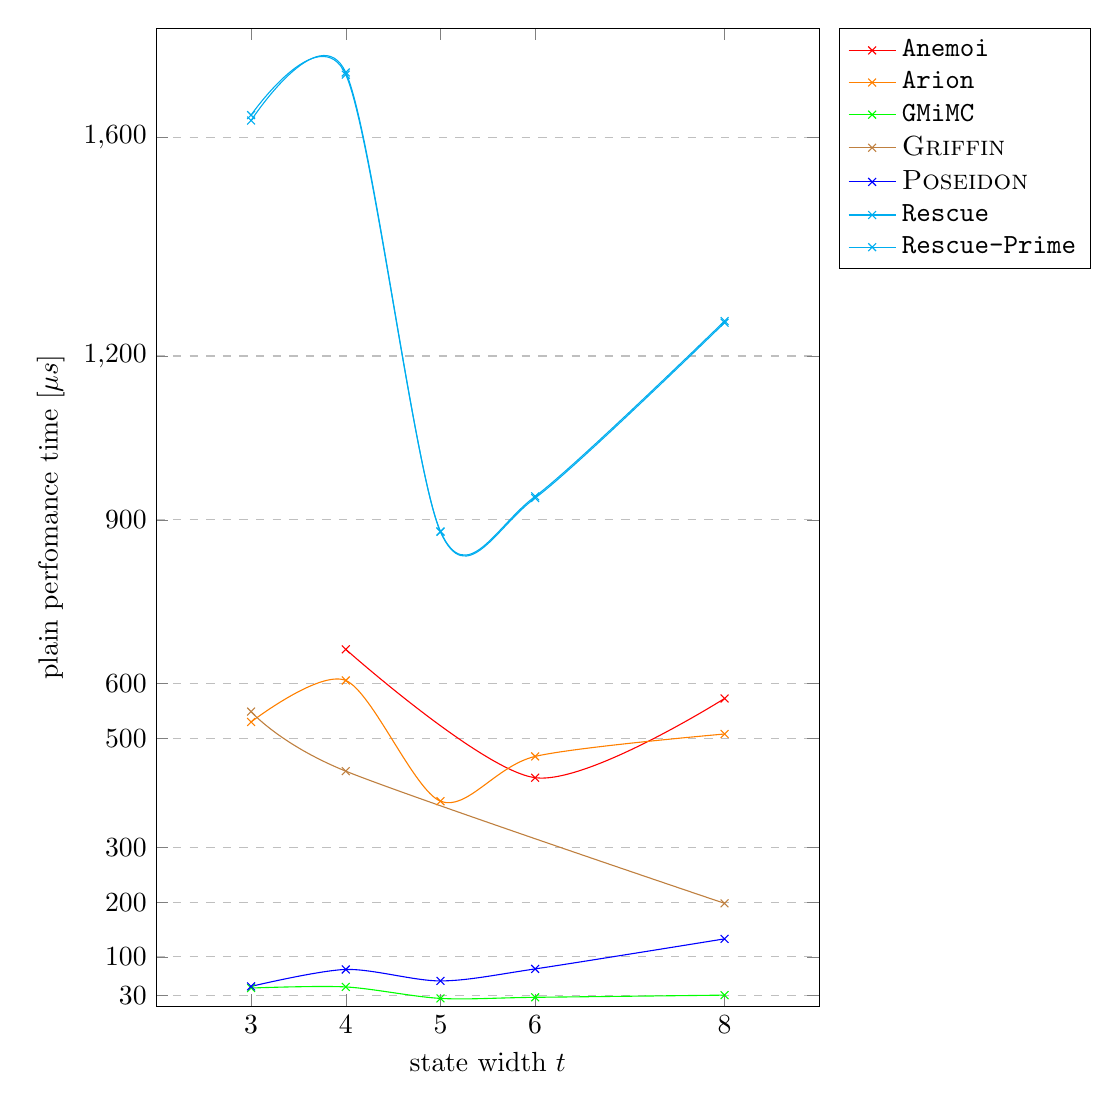
\begin{tikzpicture}
  \begin{axis}[
      xlabel={state width $t$},
      ylabel={plain perfomance time [$\mu s$]},
      ymajorgrids=true,
      grid style=dashed,
      width=10cm, height=14cm,
      xmin=2, xmax=9,
      ymin=10, ymax=1800,
      xtick={3,4,5,6,8}, ytick={30,100,200, 300, 500, 600, 900, 1200, 1600},
      legend pos=outer north east, legend cell align=left,
      smooth,
    ]

    % Anemoi
    \addplot[mark=x, color=red] plot coordinates {
        (4,663)
        (6,428)
        (8,573)
    };
    \addlegendentry{\texttt{Anemoi}}
    
    % Arion
    \addplot[mark=x, color=orange] plot coordinates {
        (3,530)
        (4,606)
        (5,385)
        (6,467)
        (8,508)
    };
    \addlegendentry{\texttt{Arion}}
    
    % GMiMC
    \addplot[mark=x, color=green] plot coordinates {
        (3,43)
        (4,45)
        (5,24)
        (6,26)
        (8,30)
    };
    \addlegendentry{\texttt{GMiMC}}
    
    \addplot[mark=x, color=brown] plot coordinates {
        (3,549)
        (4,440)
        (8,198)
    };
    \addlegendentry{\textsc{Griffin}}
    
    \addplot[mark=x, color=blue] plot coordinates {
        (3,46)
        (4,77)
        (5,56)
        (6,78)
        (8,133)
    };
    \addlegendentry{\textsc{Poseidon}}
    
    \addplot[mark=x, color=cyan] plot coordinates {
        (3,1641)
        (4,1715)
        (5,879)
        (6,943)
        (8,1264)
    };
    \addlegendentry{\texttt{Rescue}}
    
    \addplot[mark=x, color=cyan] plot coordinates {
        (3,1631)
        (4,1719)
        (5,878)
        (6,940)
        (8,1261)
    };
    \addlegendentry{\texttt{Rescue-Prime}}

  \end{axis}
\end{tikzpicture}

  \caption{Plain timing performance in $\mu s$ with $d = 5$.}\label{plot:plain}
\end{figure}

As it is possible to notice by the result's table, but even more in the plot, the fastest primitive is \texttt{GMiMC}, immediately followed by \textsc{Poseidon} and this is due to the fact that the design of these two primitives is based on keeping the computational cost of each round very low, using only low degree exponentiation in the S-Box, while having a high number of rounds.
However, the high number of rounds doesn't affect that much the performance, especially in the case of \texttt{GMiMC}, where the timings are pretty much the same for each state width.

It is also interesting the behavior of \textsc{Griffin}, in which the bigger is the state the faster is the computation and the reason behind this is that it's only done one high degree permutation per round, thus having a bigger state doesn't really affect the management of the state, while on the other hand the number of rounds is slightly lower, reducing the overall computational cost.

The remaining primitives (\texttt{Anemoi}, \texttt{Arion}, \texttt{Rescue} and \texttt{Rescue-Prime}) have an inconsistent and swinging behavior, especially \texttt{Rescue} and \texttt{Rescue-Prime}.

\section{Constraints}\label{sec:constraints}

For the second testing phase it has been analyzed the number of constraints needed both for a single round and for an entire permutation.
We analyzed also this aspect for the zero-knowledge evaluation, in order to have another point of view on the performance of the primitive other than the timings, that are exposed in the following tests \autoref{sec:proofgen} \autoref{sec:proofver}.

The general formulas to calculate the number of constraints for a single round of each primitive are the following:

\begin{align*}
  \texttt{Anemoi}_{c_r} & = c_{\text{AddRoundConstant}} + c_{\text{MixLayer}} + c_{\text{PHT}} + c_{\text{S-Box}} \\
    &= 2l + 2l^2 + 2l + 6l = 2l^2 + 10l \\
    &= \frac{t^2}{2} + 5t\\[20pt]
  \texttt{Arion}_{c_r} &= c_{\text{GTDS}} + c_{\text{MixLayer}} + c_{\text{AddRoundConstant}} \\
    &= (t-1) \cdot 7 + 16 + t + t^2 \\
    &= t^2 + 8t + 9\\[20pt]
  \texttt{GMiMC}_{c_r} &= c_{\text{ERF}} = t+2\\[20pt]
  \textsc{Griffin}_{c_r} &= c_{\text{S-Box}} + c_{\text{MixLayer}} + c_{\text{AddRoundConstant}} \\
    & = 6 + (t-2)*3 + t^2 + t \\
    & = t^2 + 4t\\[20pt]
  \textsc{Poseidon}_{c_{partial}} &= c_{\text{AddRoundConstant}} + c_{\text{S-Box}} + c_{\text{MixLayer}} \\
    &= t + 3 + t^2\\[20pt]
  \textsc{Poseidon}_{c_{full}} &= c_{\text{AddRoundConstant}} + c_{\text{S-Box}} + c_{\text{MixLayer}} \\ 
    &= t + 3t + t^2 \\
    &= t^2 + 4t\\[20pt]
  \texttt{Rescue}_{c_r} &= 2 \cdot (c_{\text{S-Box}} + c_{\text{MixLayer}} + c_{\text{AddRoundConstant}}) \\
    &= 2 \cdot (3t + t^2 + t) \\
    &= 2t^2 + 8t\\[20pt]
  \texttt{Rescue-Prime}_{c_r} &= 2 \cdot (c_{\text{S-Box}} + c_{\text{MixLayer}} + c_{\text{AddRoundConstant}}) \\
    &= 2 \cdot (3t + t^2 + t) \\
    &= 2t^2 + 8t
\end{align*}

We used the variable $c_r$ to denote the constraints per round.

Additionally, because of \textsc{Poseidon}'s design, where a round can be full or partial, we decided to show the number of constraints for both, round types and that's why for each cell there are two values, presented with the following notation \{partial\}/\{full\}, as you can see in \autoref{tab:constraintsround}.

\begin{table}[H]
  \caption{Number of constraints needed for a single round of the permutation with $d = 5$.}\label{tab:constraintsround}
  \begin{center}
    \setlength\arrayrulewidth{1pt}
    \begin{tabular}{|l|c|c|c|c|c|}
      \hline
        State width $t$ & 3 & 4 & 5 & 6 & 8 \\
      \hline
        \texttt{Anemoi} & & 28 &  & 48 & 72 \\
        \noalign{\hrule height 0.5pt}
        \texttt{Arion} & 42 & 57 & 74 & 93 & \cellcolor{orange!35} 137 \\
        \noalign{\hrule height 0.5pt}
        \texttt{GMiMC} & \cellcolor{green!35} 5 & 6 & 7 & 8 & 10 \\
        \noalign{\hrule height 0.5pt}
        \textsc{Griffin} & 21 & 32 & & & 96 \\
        \noalign{\hrule height 0.5pt}
        \textsc{Poseidon} & 15/21 & 23/32 & 33/45 & 45/60 & 75/96 \\
        \noalign{\hrule height 0.5pt}
        \texttt{Rescue} & 42 & 64 & 90 & \cellcolor{orange!35} 120 & \cellcolor{red!35} 192 \\
        \noalign{\hrule height 0.5pt}
        \texttt{Rescue-Prime} & 42 & 64 & 90 & \cellcolor{orange!35} 120 & \cellcolor{red!35} 192 \\
      \hline
    \end{tabular}
  \end{center}
\end{table}

Now we extend the above results to an entire permutation, thus we define $c_p$ as constraints per permutation and define the general formulas:
\begin{align*}
  \texttt{Anemoi}_{c_p} &= \texttt{Anemoi}_{c_r} * n + c_{\text{MixLayer}} = \texttt{Anemoi}_{c_r} * n + 2l^2 \\[20pt]
  \texttt{Arion}_{c_p} &= \texttt{Arion}_{c_r} * n + c_{\text{MixLayer}} = \texttt{Arion}_{c_r} * n + t^2 \\[20pt]
  \texttt{GMiMC}_{c_p} &= \texttt{GMiMC}_{c_r} * n \\[20pt]
  \textsc{Griffin}_{c_p} &= \textsc{Griffin}_{c_r} * n + c_{\text{MixLayer}} = \textsc{Griffin}_{c_r} * n + t^2 \\[20pt]
  \textsc{Poseidon}_{c_p} &= \textsc{Poseidon}_{c_{partial}} * n_p + \textsc{Poseidon}_{c_{full}} * n_f \\[20pt]
  \texttt{Rescue}_{c_p} &= \texttt{Rescue}_{c_r} * n \\[20pt]
  \texttt{Rescue-Prime}_{c_p} &= \texttt{Rescue-Prime}_{c_r} * n
\end{align*}

\begin{table}[H]
  \caption{Number of constraints needed for a complete permutation with $d = 5$.}\label{tab:constraintsperm}
  \begin{center}
    \setlength\arrayrulewidth{1pt}
    \begin{tabular}{|l|c|c|c|c|c|}
      \hline
        State width $t$ & 3 & 4 & 5 & 6 & 8 \\
      \hline
        \texttt{Anemoi} & & 400 & & 594 & 896 \\
        \noalign{\hrule height 0.5pt}
        \texttt{Arion} & \cellcolor{green!35} 261 & 301 & 395 & 501 & 612 \\
        \noalign{\hrule height 0.5pt}
        \texttt{GMiMC} & \cellcolor{orange!35} 1640 & \cellcolor{orange!35} 1980 & \cellcolor{orange!35} 2324 & \cellcolor{orange!35} 2672 & \cellcolor{orange!35} 3380 \\
        \noalign{\hrule height 0.5pt}
        \textsc{Griffin} & 303 & 368 & & & 928 \\
        \noalign{\hrule height 0.5pt}
        \textsc{Poseidon} & \cellcolor{orange!35} 1317 & \cellcolor{orange!35} 2104 & \cellcolor{orange!35} 2964 & \cellcolor{orange!35} 3960 & \cellcolor{red!35} 6360 \\
        \noalign{\hrule height 0.5pt}
        \texttt{Rescue} & 588 & 704 & 810 & 960 & \cellcolor{orange!35} 1536 \\
        \noalign{\hrule height 0.5pt}
        \texttt{Rescue-Prime} & 588 & 704 & 810 & 960 & \cellcolor{orange!35} 1536 \\
      \hline
    \end{tabular}
  \end{center}
\end{table}

Even though \texttt{Rescue} and \texttt{Rescue-Prime} were the two primitives with the highest number of constraints per round, if we consider the entire permutation, which is the most important aspect, these two are still in the top 3 for the highest number of constraints, but not as much as \texttt{GMiMC} and \textsc{Poseidon}.
Is immediately clear that \textsc{Poseidon} is worst in terms of number of constraints per permutation because it was already among the worst primitives considering only a round, but if we take into account its design strategy, it's obvious that the number of constraints per permutations increase exponentially due to its high number of rounds.

Furthermore, even though \texttt{GMiMC} is the second worst's primitive, it's not a bad result considering that the number of rounds needed by \texttt{GMiMC} is almost double of those needed by \textsc{Poseidon}.

On the other hand, thanks to its design that allow to keep the number of rounds very low, \texttt{Arion} is the best primitive in terms of constraints per permutation, even though it wasn't the best in terms of constraints per round.

\section{Proof generation}\label{sec:proofgen}

In the third test type, we focused on the time needed to generate a zero-knowledge proof with the Plonk constraint system, which we have collected in the \autoref{tab:proofgen} and then plotted in the \autoref{plot:proofgen} for having a visual comparison.

\begin{table}[H]
  \caption{Proof generation performance's time in $ms$ with $d = 5$.}\label{tab:proofgen}
  \begin{center}
    \setlength\arrayrulewidth{1pt}
    \begin{tabular}{|l|c|c|c|c|c|}
      \hline
        State width $t$ & 3 & 4 & 5 & 6 & 8 \\
      \hline
        \texttt{Anemoi} & & 659 &  & 658 & 659 \\
        \noalign{\hrule height 0.5pt}
        \texttt{Arion} & 358 & 660 & 356 & \cellcolor{green!35} 355 & 657 \\
        \noalign{\hrule height 0.5pt}
        \texttt{GMiMC} & \cellcolor{orange!35} 1962 & \cellcolor{red!35} 3719 & \cellcolor{orange!35} 2160 & \cellcolor{orange!35} 1972 & \cellcolor{orange!35} 1982 \\
        \noalign{\hrule height 0.5pt}
        \textsc{Griffin} & 655 & 657 & & & 660 \\
        \noalign{\hrule height 0.5pt}
        \textsc{Poseidon} & \cellcolor{orange!35} 1958 & \cellcolor{orange!35} 1961 & \cellcolor{orange!35} 1973 & \cellcolor{orange!35} 1959 & \cellcolor{red!35} 3719 \\
        \noalign{\hrule height 0.5pt}
        \texttt{Rescue} & \cellcolor{orange!35} 1221 & \cellcolor{orange!35} 1212 & 659 & 664 & \cellcolor{orange!35} 1219 \\
        \noalign{\hrule height 0.5pt}
        \texttt{Rescue-Prime} & \cellcolor{orange!35} 1212 & \cellcolor{orange!35} 1219 & 659 & 659 & \cellcolor{orange!35} 1213 \\
      \hline
    \end{tabular}
  \end{center}
\end{table}

\begin{figure}[H]
  \hspace{60pt}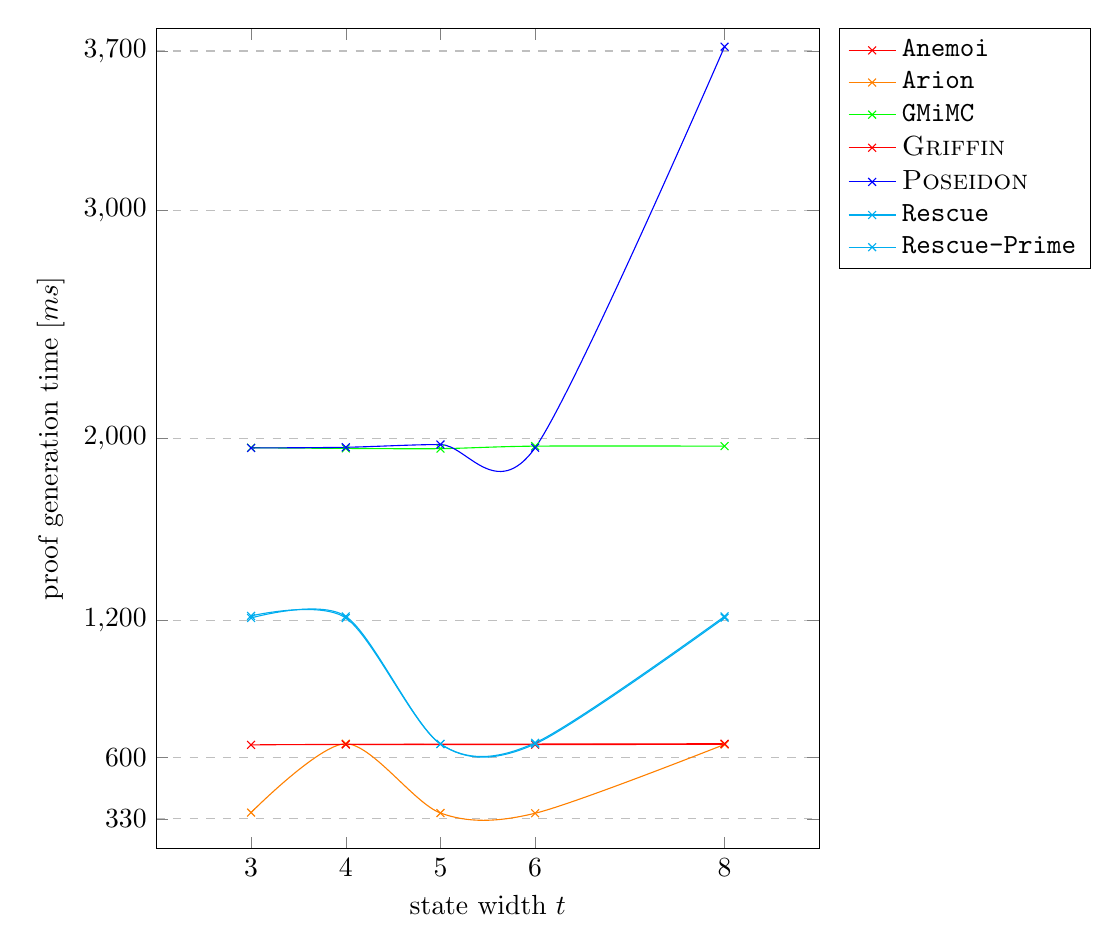
\begin{tikzpicture}
  \begin{axis}[
      xlabel={state width $t$},
      ylabel={proof generation time [$ms$]},
      ymajorgrids=true,
      grid style=dashed,
      width=10cm, height=12cm,
      xmin=2, xmax=9,
      ymin=200, ymax=3800,
      xtick={3,4,5,6,8}, ytick={330,600,1200,2000,3000, 3700},
      legend pos=outer north east, legend cell align=left,
      smooth,
    ]
      
    % Anemoi
    \addplot[mark=x, color=red] plot coordinates {
        (4,657)
        (6,656)
        (8,658)
    };
    \addlegendentry{\texttt{Anemoi}}
    
    % Arion
    \addplot[mark=x, color=orange] plot coordinates {
        (3,358)
        (4,660)
        (5,356)
        (6,355)
        (8,657)
    };
    \addlegendentry{\texttt{Arion}}
    
    % GMiMC
    \addplot[mark=x, color=green] plot coordinates {
        (3,1959)
        (4,1956)
        (5,1955)
        (6,1966)
        (8,1966)
    };
    \addlegendentry{\texttt{GMiMC}}
    
    \addplot[mark=x, color=red] plot coordinates {
        (3,655)
        (4,657)
        (8,660)
    };
    \addlegendentry{\textsc{Griffin}}
    
    \addplot[mark=x, color=blue] plot coordinates {
        (3,1958)
        (4,1961)
        (5,1973)
        (6,1959)
        (8,3719)
    };
    \addlegendentry{\textsc{Poseidon}}
    
    \addplot[mark=x, color=cyan] plot coordinates {
        (3,1221)
        (4,1212)
        (5,659)
        (6,664)
        (8,1219)
    };
    \addlegendentry{\texttt{Rescue}}
    
    \addplot[mark=x, color=cyan] plot coordinates {
        (3,1212)
        (4,1219)
        (5,659)
        (6,659)
        (8,1213)
    };
    \addlegendentry{\texttt{Rescue-Prime}}

  \end{axis}
\end{tikzpicture}

  \caption{Proof generation performance's time in $ms$ with $d = 5$.}\label{plot:proofgen}
\end{figure}

For a better understanding of the results, we decided to assign the same color to \texttt{Anemoi} and \textsc{Griffin} and also to \texttt{Rescue} and \texttt{Rescue-Prime}, because their timings are so close that their curves are overlapping.

As it is possible to evince from these results, the fastest primitive for this category of tests is \texttt{Arion}, immediately followed by \texttt{Anemoi} and \textsc{Griffin}.
Nonetheless, considering that the latest two primitives work only with 3 out 5 possible state widths, their results are almost as good as \texttt{Arion}.
If we have to take also in consideration the stability of the results, \texttt{Arion} is a little unstable and whose behavior is closely related to the one of the plain performance test.

On the other spectrum of the tests' results, \textsc{Poseidon} is the worst primitive in terms of proof generation as expected by the high number of constraints per permutation highlighted in the previous \autoref{sec:constraints}, almost doubling the time in the case of state width $t = 8$ respectively to average time of the other state widths' values.

\section{Proof verification}\label{sec:proofver}

In the last category of tests we focused on the verification process of the constraint generated in the Plonk system, and the results have been pretty much the same, around $7.26\pm0.03\ [ms]$ independently of the state width, for all the primitives.
Due to these results, it has been decided to not show any table or plot like in the previous sections.

\chapter{Conclusion}\label{chap:conclusion}

In conclusion, as it was possible to deduct from the tests, the design strategy for primitives plays a key role in how the function behaves with different parameters, highlighting the strengths and weaknesses of each one.
This is a crucial step before proceeding with the optimization of these permutation functions, because it's beneficial to decide which applications can fit better the behavior of the primitive, not only from a performance standpoint, but even more from a security one.
For example, even though \texttt{Arion} is the fastest for a certain choice of parameters, it leads to the same results of \texttt{Anemoi} and \textsc{Griffin} for others, thus if an application needs among the requirements also a certain level of stability in the performances while providing a broader choice of parameters, going with \texttt{Arion} would not be the best choice.
On the other hand, while \texttt{GMiMC} has been one of the first primitives that animated some interest in AO cryptography, thus one may think that its performance will not be as good as the newly proposed primitives, if the area of application needs a higher number of hashes computations without the constant need of zero-knowledge proofs, \texttt{GMiMC} would be the best choice.

We hope that with this paper we have provided a good overview of the current state of the AO primitives and that with these results new optimizations may come out, or even better that this will spark new ideas for innovative design strategies that will enrich the cryptographic community.

\chapter{References}

\nocite{*}
\printbibliography[heading=subbibnumbered, title={Bibliography}]

\newpage
\section{List of Figures}\label{sec:listoffigures}
\listoffigures

\newpage
\section{List of Tables}\label{sec:listoftables}
\listoftables

%\newpage
%\section{List of Algorithms}\label{sec:listofalgorithms}
\listofalgorithms

\end{document}
